\def\paperRoman{II}
\documentclass[10pt,a4paper]{article}
\usepackage[margin=22mm,top=23mm,bottom=23mm]{geometry}
\usepackage{fontspec}
\setmainfont{Latin Modern Roman}
\setsansfont{DejaVu Sans}
\usepackage{babel}
\babelprovide[import,main]{spanish}
\usepackage{amsmath,amssymb}
\usepackage{unicode-math}
\setmathfont{Latin Modern Math}
\usepackage{graphicx,booktabs,longtable,array,enumitem,xcolor,fancyhdr,xurl,hyperref,tikz,microtype}
\usetikzlibrary{arrows.meta,positioning}
\definecolor{navy}{HTML}{17375C}
\definecolor{teal}{HTML}{0F8F86}
\definecolor{gold}{HTML}{B28B3C}
\hypersetup{colorlinks=true,linkcolor=navy,urlcolor=teal,citecolor=navy,pdfauthor={Juan Manuel Goenaga Castro}}
\setlength{\parindent}{0pt}
\setlength{\parskip}{5.2pt}
\linespread{1.07}
\setlist{nosep,leftmargin=1.5em,topsep=4pt}
\setlength{\headheight}{15pt}
\pagestyle{fancy}
\fancyhf{}
\fancyhead[L]{\sffamily\footnotesize GoToGym Quantum Research}
\fancyhead[R]{\sffamily\footnotesize Serie QAF audiovisual / \paperRoman}
\fancyfoot[L]{\sffamily\scriptsize Prepublicación metodológica / 22 de octubre de 2026}
\fancyfoot[R]{\sffamily\footnotesize\thepage}
\renewcommand{\headrulewidth}{0.4pt}
\newcommand{\papertitle}[3]{\begin{center}\sffamily\small\textcolor{teal}{MANUSCRITO #1 / ARQUITECTURA AUDIOVISUAL QAF}\par\vspace{9pt}{\huge\bfseries\textcolor{navy}{#2}}\par\vspace{7pt}{\large #3}\par\vspace{11pt}{\normalsize\bfseries Juan Manuel Goenaga Castro}\par\small GoToGym Quantum Research / Bogotá D.C., Colombia\par\small 22 de octubre de 2026 / Versión 1.0\end{center}\vspace{4pt}}
\newcommand{\status}[1]{\noindent\colorbox{navy!7}{\parbox{0.966\linewidth}{\small\textbf{Naturaleza del trabajo.} #1}}\par\vspace{6pt}}
\newcommand{\keywords}[1]{\textbf{Palabras clave:} #1.}
\newcommand{\R}{\mathbb{R}}
\newcommand{\C}{\mathbb{C}}
\newcommand{\tr}{\operatorname{Tr}}
\newcommand{\diag}{\operatorname{diag}}
\newcommand{\argmin}{\operatorname*{arg\,min}}
\newcommand{\argmax}{\operatorname*{arg\,max}}
\newcommand{\IP}{\mathcal{I}}
\newcommand{\sectionpage}[1]{\clearpage\section{#1}}
\newcommand{\compacttable}{\small\renewcommand{\arraystretch}{1.22}}
\emergencystretch=2em

\begin{document}
\papertitle{II}{Cinematografía computacional y narrativa verificable}{Control de cámara, atención, identidad de marca y montaje de un minuto}
\status{Modelo de dirección y planificación. Incluye una verificación de trayectoria de cámara; las hipótesis de percepción y eficacia de marca requieren evaluación humana.}
\begin{abstract}
Se formula la dirección cinematográfica de videos explicativos como un problema jerárquico de restricciones y preferencias. El nivel superior fija propósito, audiencia, evidencia y transformación narrativa; el nivel intermedio selecciona planos y relaciones; el inferior determina encuadre, cámara, iluminación, tipografía y montaje. Se introducen una utilidad multiobjetivo, un grafo de continuidad y una discretización exacta en cuadros. Se deriva una trayectoria de cámara de mínimo jerk con condiciones de posición, velocidad y aceleración en los extremos, y se especifica una interpolación de orientación que evita discontinuidades. La marca se representa mediante tokens y decisiones de composición, conservando por separado información visual y evidencia de producto. El caso de diseño es una película de running donde el descanso declarado cambia la propuesta. Se propone un experimento que compara montaje fijo, planificación clásica y planificación relacional QAF con los mismos recursos. El objetivo es hacer reproducible la dirección sin reducir la calidad artística a una puntuación automática.
\end{abstract}
\keywords{cinematografía computacional, narrativa, control óptimo, atención, montaje, identidad de marca}

\section{De una intención creativa a un contrato ejecutable}
La dirección se inicia con cuatro preguntas: quién necesita decidir, qué dificultad reconoce, qué capacidad interviene y qué acción queda disponible. Una película de un minuto debe permitir responderlas sin una explicación posterior del productor. El contrato editorial incluye una promesa, una demostración, una limitación pertinente y un llamado a la acción. Las capas futuristas muestran relaciones entre información y decisión; el protagonista mantiene la experiencia humana.

El estilo propuesto combina entornos reconocibles, luz motivada, textura material y visualización de información. ``Ciencia ficción plausible'' significa que los recursos conceptuales pueden exceder la apariencia actual de la interfaz, siempre que no atribuyan mediciones o automatizaciones inexistentes. El brillo de un holograma no acredita una señal biométrica. Un plano de una rodilla no debe convertirse en un supuesto escáner diagnóstico si la entrada real es un formulario.

La línea de producción conserva propósito, audiencia y etapa comercial como variables distintas. Reconocimiento, consideración, conversión y fidelización pueden requerir finales diferentes. No se optimizan simultáneamente como si tuvieran el mismo denominador. Una mejora de comprensión puede ser un objetivo inicial más próximo a la película explicativa que ventas o retención a largo plazo.

\section{Modelo jerárquico de la película}
Sea $S=(s_1,\ldots,s_n)$ una secuencia de planos y $a_i$ su función narrativa. Definimos las funciones permitidas: situación, problema, mecanismo, demostración, beneficio y acción. Una gramática $\mathcal G$ restringe transiciones y exige que un mecanismo afirmado tenga evidencia o un rótulo conceptual compatible. La gramática admite varias películas válidas; no fija una única estética.

La decisión se plantea como optimización multiobjetivo:
\begin{equation}
 \max_S\ \left(U_{\mathrm{comprensión}},U_{\mathrm{marca}},U_{\mathrm{emoción}},-C_{\mathrm{producción}},-R_{\mathrm{confusión}}\right)
 \quad\text{sujeto a }S\in\mathcal G\cap\mathcal F.
\end{equation}
$\mathcal F$ contiene duración, derechos, evidencia, accesibilidad y factibilidad física. Cuando se usa escalarización, $J=\sum_kw_k\widetilde U_k$ emplea pesos preespecificados y análisis de sensibilidad. Se conserva también la frontera de Pareto: una pequeña ganancia estética no autoriza violar una restricción de veracidad.

La representación QAF del manuscrito I es candidata para interacciones entre planos, no requisito para medir cada utilidad. Un comparador clásico debe recibir los mismos nodos, aristas, etiquetas y condiciones de producción. Si se descubre que una función aditiva explica la decisión igual de bien, se conserva la solución más simple.

\section{Tiempo, lectura y continuidad}
El tiempo editorial es racional. A 30 cuadros por segundo, un episodio de 60 segundos contiene $F=1.800$ cuadros. Para planos sin solape, $\sum_if_i=F$, con $f_i\in\mathbb N$. Para transiciones superpuestas de $o_i$ cuadros:
\begin{equation}
 F=\sum_{i=1}^nf_i-\sum_{i=1}^{n-1}o_i.
\end{equation}
Las duraciones de voz, texto y transición se computan sobre el resultado final. Un final de seis segundos que contiene una disolución de dos no dispone necesariamente de seis segundos completos de lectura.

Para un bloque de texto con $c_i$ caracteres y velocidad máxima de diseño $r_{\max}$, se exige inicialmente $f_i\geq\lceil30c_i/r_{\max}\rceil$. $r_{\max}$ se obtiene mediante pruebas con la audiencia, idioma y tamaño de pantalla. Las siglas desconocidas y el texto técnico aumentan la dificultad más que la cuenta de caracteres. El límite mecánico se complementa con revisión de lectura real.

La continuidad se organiza mediante un grafo. Para planos adyacentes se penalizan cambios de eje, dirección de mirada, identidad, vestuario y posición del objeto principal. Se define
\begin{equation}
 C_{\mathrm{continuidad}}=\sum_i\sum_k\alpha_k\,d_k(s_i,s_{i+1}),
\end{equation}
con distancias específicas por atributo. Un cambio de eje deliberado puede ser válido si comunica una ruptura; el modelo debe permitir excepciones documentadas. La continuidad corporal y del producto se verifica visualmente; una similitud de embeddings no garantiza anatomía correcta.

\section{Geometría de cámara y movimiento}
La cámara se describe por intrínsecos $K_c$, rotación $R$ y traslación $t$. La proyección de un punto tridimensional $X$ es
\begin{equation}
 \lambda\begin{bmatrix}u&v&1\end{bmatrix}^{T}=K_c[R\mid t]\begin{bmatrix}X^T&1\end{bmatrix}^{T}.
\end{equation}
Se fijan convención de ejes, unidades, tamaño de sensor y recorte. La focal aparente de 35, 50 u 85 mm es una guía creativa; cuando no existe cámara física no se registra como EXIF real. Un recorte digital no cambia la perspectiva si no cambia el centro de proyección.

Una trayectoria entre posiciones $p_0$ y $p_1$ durante $T$ segundos puede minimizar
\begin{equation}
 J_{\mathrm{mov}}=\int_0^T\|\dddot p(t)\|^2\,dt,
\end{equation}
con posición fijada y velocidad/aceleración nulas en ambos extremos. La ecuación de Euler--Lagrange conduce a una trayectoria polinómica de grado cinco. Con $u=t/T$:
\begin{align}
 s(u)&=10u^3-15u^4+6u^5,\\
 p(t)&=p_0+(p_1-p_0)s(t/T),\\
 J_{\mathrm{mov}}&=720\frac{\|p_1-p_0\|^2}{T^5}.
\end{align}
El último resultado evidencia que acortar una maniobra aumenta fuertemente su coste de suavidad. No determina por sí mismo si el movimiento cuenta bien una historia. Las condiciones no incluyen obstáculos, velocidad máxima o visibilidad; con esas restricciones se resuelve un control óptimo o spline restringido.

Para orientación se utiliza interpolación esférica entre cuaterniones unitarios:
\begin{equation}
 q(u)=\frac{\sin((1-s(u))\theta)}{\sin\theta}q_0+
 \frac{\sin(s(u)\theta)}{\sin\theta}q_1.
\end{equation}
Se invierte el signo de un extremo si el producto escalar es negativo para tomar la trayectoria corta; cerca de $\theta=0$ se usa una aproximación estable y renormalización. Con posición y orientación se inspeccionan horizontes, oclusión y cortes de sujeto. Una cámara suave puede seguir una trayectoria visualmente incorrecta.

\begin{figure}[ht]\centering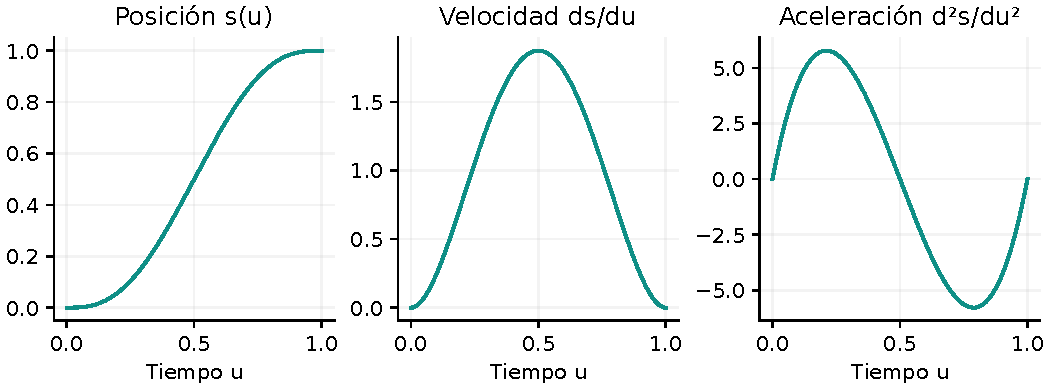
\includegraphics[width=.82\linewidth]{figures/camera_minimum_jerk.pdf}\caption{Posición, velocidad y aceleración normalizadas del polinomio. El control adjunto verifica condiciones en extremos y coste de jerk 720 en tiempo unitario.}\end{figure}

\section{Iluminación, espacio y composición}
Cada escena declara fuente principal motivada, relleno, separación y exposición. Las relaciones de iluminación se eligen para conservar piel, ropa y lectura de pantalla. Los parámetros se expresan en el sistema del motor y se calibran con referencias; no se inventa una conversión universal de un deslizador de potencia a lux sobre el sujeto. La luz de una ventana o pantalla debe ser espacialmente compatible con el entorno.

Una exposición simplificada depende de luminancia, tiempo de exposición y apertura. El ángulo de obturación relaciona cuadro y tiempo: $t_e=\theta_s/(360f_r)$, donde $f_r$ es la frecuencia de cuadros. A 30 fps y $\theta_s=180^\circ$, $t_e=1/60$ s. Es una elección creativa de partida, no obligación universal. La generación de imágenes y los overlays deben mantener desenfoque de movimiento compatible con la toma base.

La composición define máscaras de exclusión para rostro, manos, producto, acción y subtítulos. Cada capa crítica $M_k$ debe satisfacer restricciones de área y solape. Un ejemplo es $|M_{\mathrm{texto}}\cap M_{\mathrm{rostro}}|=0$ cuando no haya justificación editorial. El contraste se mide en la imagen compuesta, no solamente en el color de texto sobre un fondo ideal. Las escenas vertical y horizontal reciben encuadres propios, no una simple copia con barras.

El color se separa en identidad y apariencia. Los tokens recibidos incluyen grafito \#101012, esmeralda \#1A9B76, zafiro \#17375C, dorado \#D4B46A y turquesa \#0FBFB0. Los acentos adicionales de campaña permanecen provisionales. Las transformaciones de visualización pueden modificar la apariencia de un color; los elementos gráficos de marca se revisan tras la transformación y la compresión, con el tratamiento descrito en el manuscrito III.

\section{Atención y accesibilidad como hipótesis medibles}
Se propone un modelo de carga por plano $\ell_i=\beta_1N_{\mathrm{conceptos}}+\beta_2N_{\mathrm{objetos}}+\beta_3v_{\mathrm{texto}}+\beta_4m_{\mathrm{cámara}}$. Los coeficientes deben aprenderse o calibrarse sobre tareas de comprensión; no se presentan como una ley neurocientífica. Saliencia, interés y comprensión no son equivalentes. Un estímulo llamativo puede aumentar fijaciones y reducir recuerdo del mecanismo.

Los criterios WCAG sirven como referencia de accesibilidad para subtítulos, contraste y destellos en publicación web \cite{wcag}. Su aplicación al video se evalúa en la composición final y el reproductor de destino. No basta con incluir una pista de subtítulos vacía o texto inaccesible por tamaño. Se revisan hablantes, sonidos relevantes, sincronía y lectura a escala móvil; la información esencial no depende exclusivamente del color.

La evaluación contempla tres tareas: identificar el problema humano, explicar en una frase qué hace el sistema y distinguir una función disponible de una visualización conceptual. Se añade recuerdo diferido y una pregunta de siguiente paso. La puntuación estética se recoge aparte para no confundir agrado con exactitud.

\section{Caso de diseño: running con contexto}
El piloto parte de una comprobación local de la versión auditada del motor: con un contexto sintético válido que incluye 20 minutos disponibles y cinco horas de sueño, se devuelve caminata de 15 minutos. Los otros campos del fixture también importan. La secuencia no afirma que dormir cinco horas determine siempre esa salida.

\begin{table}[ht]\centering\compacttable
\begin{tabular}{p{.12\linewidth}p{.25\linewidth}p{.50\linewidth}}\toprule
Tiempo & Función & Decisión de dirección \\\midrule
0--5 s & Situación & Detalle de zapatillas; acción humana antes de explicación.\\
5--13 s & Contexto & Persona reconoce cansancio; datos declarados rotulados como ejemplo.\\
13--27 s & Mecanismo & Entradas y opciones; gráfico conceptual sin sensado corporal ficticio.\\
27--43 s & Demostración & Resultado pendiente de decisión; caminata como dramatización.\\
43--54 s & Alcance & La propuesta puede cambiar; no se analiza video de running.\\
54--60 s & Marca y acción & Logo original y un siguiente paso legible.\\\bottomrule
\end{tabular}\caption{Diseño narrativo inicial; no constancia de rodaje o recorrido autenticado.}
\end{table}

El montaje usa sonido ambiente para presencia, un acercamiento al reconocer el contexto y un plano estable para la propuesta. La interfaz recreada se identifica como conceptual. El actor no representa una mejora clínica. La toma de caminata no acredita que un usuario aceptó o completó la sesión. Estas distinciones permiten un relato atractivo sin degradar la evidencia.

\section{Experimento propuesto y criterio de falsación}
Se comparan tres condiciones con el mismo banco de tomas: plantilla fija, planificador clásico con grafo de continuidad y planificador relacional QAF. Se equilibran contenido, duración, voz, presupuesto y audiencia. Las versiones se asignan aleatoriamente y las evaluaciones se realizan a ciegas respecto al método. El desenlace primario es comprensión de mecanismo; los secundarios son recuerdo, credibilidad, estética y coste de revisión.

La hipótesis queda refutada operacionalmente si no existe mejora relevante o si el coste adicional elimina su utilidad. Se registra también daño por confusión: porcentaje de personas que atribuye al producto una capacidad no demostrada. Una película que gana agrado y aumenta esa confusión no cumple el objetivo.

\section{Conclusión}
La contribución es convertir decisiones creativas en contratos editables, restricciones y controles observables, preservando espacio para dirección artística. La trayectoria de cámara tiene una verificación matemática; la narrativa y la marca requieren pruebas con espectadores. El sistema será de nivel profesional cuando las decisiones puedan revisarse, repetirse y producir películas cuya calidad se sostenga en evaluación, no cuando acumule nombres de algoritmos.

\begin{thebibliography}{E3}
\bibitem[Q1]{q1} Goenaga, J. M. (2025). \emph{Quantum Analysis Frameworks}. Documento aportado.
\bibitem[Q5]{q5} Goenaga, J. M. (2026). \emph{Consolidated Experimental Evidence for QAF}. Documento aportado.
\bibitem[E1]{wcag} W3C. \emph{Web Content Accessibility Guidelines 2.2}. Recomendación de 12/12/2024, consulta 22/10/2026. \url{https://www.w3.org/TR/WCAG22/}.
\bibitem[E2]{otio} Academy Software Foundation. OpenTimelineIO, documentación primaria: estructura de línea de tiempo y medios referenciados. Consulta 22/10/2026. \url{https://opentimelineio.readthedocs.io/en/latest/index.html}.
\bibitem[I1]{audit} GoToGym. \emph{Auditoría para la serie audiovisual}. Registro local del commit \texttt{6d2e95d}, escenarios sintéticos y límites de validación, 22/10/2026. Se incluye en el paquete antecedente Studio v2.
\end{thebibliography}
\end{document}
